%-----------------------------------------------%
% Packages arranged by : Tsz Timmy Chan	        %
%                 Date : Apr 17th, 2020	        %
%	See ICLSpreamble.sty for details	        %
%	Uses biblatex-apa package for references    %
%-----------------------------------------------%
% File hosted on Overleaf and synced with Github

\documentclass{ICLSarticle} % Custom formatting file, based on standard article class
\usepackage{ICLSpreamble}   % Cusom commands defined here, as well as useful packages.

\ICLStitle{Assignment 1: Boundness of Multi-Armed Bandits}
% Work Title Here.

% YOUR NAME(S) HERE 
\author{XU Guosong, 20830011, gxuae@connect.ust.hk \and CHEN Zuozhi, 20797609, zchenfu@connect.ust.hk%

(
GitHub Link: https://github.com/LegendreXu/ReinforcementLearning/tree/main/MAB)
\vspace{-10ex}} %removes spacing after authors


\addbibresource{library.bib}		% Reference file, NO SPACES in the name


% CUSTOM PACKAGES GO HERE %
%\usepackage{LSRIcommon}
% CUSTOM PACKAGES GO HERE %

\begin{document}

%====ABSTRACT AND KEYWORDS====%
\maketitle
\begin{ICLSabstract}
	\documentclass{article}
\usepackage[utf8]{inputenc}

\title{     }
\author{     }
\date{     }

\begin{document}
Over recent decades, we have seen multi-bandits algorithms is widely applied in modeling the explore-exploit tradeoff. Although we do not agree that this dilemma exists when one makes investing decision by the nature of the stock market, we would like to have experimental research on the backtesting result of MAB algorithms. The report begins by discussing the application of the multi-bandits algorithm on stock selection and compares them with other traditional investing strategies. It then further investigate the deficiency of the MAB algorithm and potential solution.

\end{document} % This template includes standalone package so this works nicely
\end{ICLSabstract}
%	\ICLSkeywords{maximum five keywords should be included}




%====MAIN TEXT BELOW====%
\documentclass{article}
\usepackage[utf8]{inputenc}

\title{     }
\author{     }
\date{     }

\addbibresource{library.bib}
\begin{document}

\section{Theoretical Formulation}
\subsection{Multi-Bandits Problem} 
K-armed bandit problem is equivalent with K-step Markov Decision Process, but it is not a perfect solution for the real world stock selection.
As we all know, bandit problem is to minimize the regret:
$$
\rho = Tq^*-\sum\limits_{t=1}^{T}\hat{r_t}
$$
where $q^*=\max\limits_{k}\{q_k\}$ is the maximal reward expectation, and $\hat{r_t}$ is the realized reward in round  $t$.
That leads the "explore-exploit dilemma":
\begin{itemize}
    \item  Explore: $q_i = \frac{\sum \hat{r_{i,t}}}{k}$ we perform $k-$th observation and $q_i \to q^*$ when $k \to \infty$.
    \item  Exploit: take $\max\{q_1,q_2,\dots,q_K\}$ to maximize the reward.
    \end{itemize}
\subsection{Natural Deficiencies of MAB on Stock Market}    
But this problem DO NOT fit the stock market:
First, the bandit problem does not make use of all available information: we do not need to buy a stock to observe its return. Second, each trial on the bandit problem is exactly identical for the player, but an investor can always make a new decision when he keeps his current position.
    
\subsection{Problem Formulation and Intuitive View}
We would like to explore whether multiple arm bandits can help us select stocks. We assume that every stock can be treated as an arm with different daily returns. Then we expect the bandit algorithm can adapt itself to the market based on the return of the selected stocks previously. Furthermore, we make the assumption that there are no transaction costs, no slippage, and we can buy any share of stocks. Besides, we liquidate our position day-to-day.
In order to evaluate the performance of the bandits method, we compare it with the equal-weighted strategy which simply buys equal amounts of stocks in the responding universe, and a simple advanced momentum strategy that chases the stock with high momentum.   
Initially, we believe that the performance of bandits will be similar to the equal-weighted one, but worse than the momentum one. This intuitive view is verified in our experiment, which is consistent with our assumption that MAB can not be a useful strategy to select stocks.
Then we would like to compare the bandit algorithm with simple traditional strategies on historical data.
\section{Methodology}
\subsection{Data Set}
We selected daily close prices of 48 US stocks from 2016/01/04 to 2022/03/04(see the list on GitHub), and 45 European stocks, from 2010/01/04 to 2019/12/30(STOXX50 Index except 5 stock without enough data) as our data set. 
\subsection{MAB Strategies}
\subsubsection{$\epsilon$ greedy}
Choose to "explore" a random stock with probability $\epsilon$ or choose to "exploit" base on current estimation with probability $1-\epsilon$.
\subsubsection{Gradient Bandits}
We define a preference for choosing an arm $H_t(a)$:
$$Pr(A_t=a)=\frac{\exp(H_t(a))}{\sum\limits_{b=1}^{K}\exp(H_t(b))}=\pi_t(a)$$
\subsubsection{Upper Confidence Bound}
As we claimed,  $q_i \to q^*$ when $k \to \infty$. But with finite observations, we believe that the error of estimation $\text{error}=|\hat q_i-q_i|$ is small with a high probability.
With Chernoff-Hoffeding bound, we have that
$$
Pr(\text{error}=|\hat q_i-q_i|\leq \sqrt{\frac{2\ln T}{k}})\geq	1-\frac{2}{T^4}
$$
Then we maximize the Upper Confidence Bound instead of the estimation to choose the stock.
\subsection{Traditional Strategies}
\subsubsection{Equal Weighted Portfolio}
Regardless of the asset, all $M$ stocks are directly placed into equal money: 
$$W_{EW} = \frac{\text{budget}}{M}$$
\subsubsection{Adjusted Momentum Factor}
We established a simple momentum factor:
$$f = \mu- \sigma$$
where $\mu$ is the time-series average of daily return and $\sigma$ is the time-series standard deviation of daily return. We use 120 trading days as look-back period and select the stock with highest factor value every 20 trading days.

\section{Numerical Results}
We perform simple back-testing for the two traditional strategies, but inevitable randomness exists for the three MAB strategies. Hence, we use Monte Carlo simulation to get a distribution of the performance of MAB strategies. We can only present the most vital data due to the page limit, you can find more detailed result on the "results.ipynb" of our GitHub repo.

\subsubsection{Summary of Back-test}
First, we compare key indicators of different strategies: Annualized Return, Aunnalized Volatility, Downside Deviation, Max Drawdown in percentage terms, Max Drawdown in dollars,  Sharpe ratio, and Sortino ratio. (See Table 1 & 2)
As for the three MAB strategies, we use the average value of 500 times simulation.

\begin{table}[H]
\caption{An overview of the back-test result on US market}
\centering
\begin{tabular}{|c | c | c | c | c | c | }
\hline
\multirow{2}{*}{Indicator} & \multicolumn{2}{c|}{Traditional}&\multicolumn{3}{c|}{Multi-Armed Bandits}  \\ \cline{2-6}
& Momentum & Equal Weighted & $\epsilon$ greedy & Gradient & UCB  \\ \hline  
Return & 0.311164 & 0.162573 & 0.093669 & 0.124347 & 0.121693  \\ \hline
Volatility & 0.361366 & 0.198137 & 0.331763 & 0.315594 & 0.312371  \\ \hline
Downside Risk & 0.253928 & 0.139940 & 0.195906 & 0.188475 & 0.189206  \\ \hline
MDD(pct) & 0.171664 & 0.315327 & 0.293719 & 0.311644 & 0.331689  \\ \hline
MDD(dollar) & 2.385027 & 0.607451 & 1.116377 & 1.045958 & 1.011529  \\ \hline
Sharpe & 0.861077 & 0.82050 & 0.338658 & 0.449481 & 0.436186  \\ \hline
Sortino & 1.22540 & 1.161731 & 0.494220 & 0.687214 & 0.664635  \\ \hline
\end{tabular}
\end{table}
\begin{table}[H]
\caption{An overview of the back-test result on EU market}

\centering
\begin{tabular}{|c | c | c | c | c | c | }
\hline
\multirow{2}{*}{Indicator} & \multicolumn{2}{c|}{Traditional}&\multicolumn{3}{c|}{Multi-Armed Bandits}  \\ \cline{2-6}
& Momentum & Equal Weighted & $\epsilon$ greedy & Gradient & UCB  \\ \hline  
Return & 0.103070 & 0.120219 &  0.088928 & 0.074552 & 0.072108  \\ \hline
Volatility & 0.278810 & 0.176927 & 0.257559 & 0.259310 & 0.258847  \\ \hline
Downside Risk & 0.209661 & 0.128526 & 0.187814 & 0.186711 & 0.186903  \\ \hline
MDD(pct) & 0.221765 & 0.326124 & 0.349639 & 0.343982 & 0.338483  \\ \hline
MDD(dollar) & 1.687033 & 0.504843 & 1.041196 & 0.945552 & 0.940655  \\ \hline
Sharpe & 0.369679 & 0.679486 & 0.344047 & 0.278499 & 0.287985  \\ \hline
Sortino & 0.491604 & 0.935368 & 0.473899 & 0.389044 & 0.403598  \\ \hline
\end{tabular}
\end{table}

\subsubsection{Distribution of MAB returns}
\begin{figure}[H]
\begin{center}
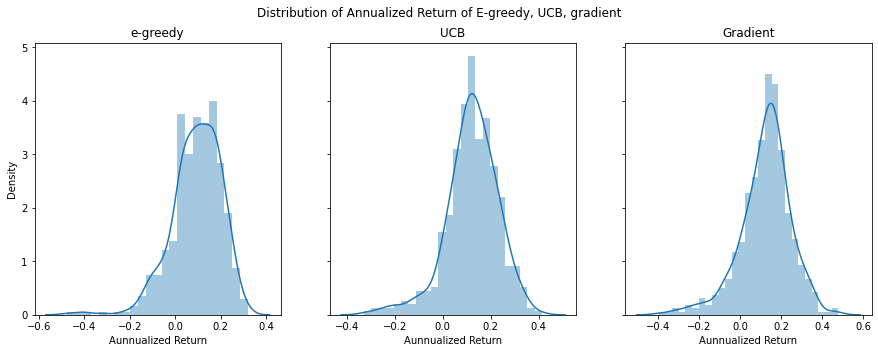
\includegraphics[width=.6\textwidth]{us}
\end{center}
\caption{The distribution of returns on US market}
\end{figure}


\begin{figure}[H]
\begin{center}
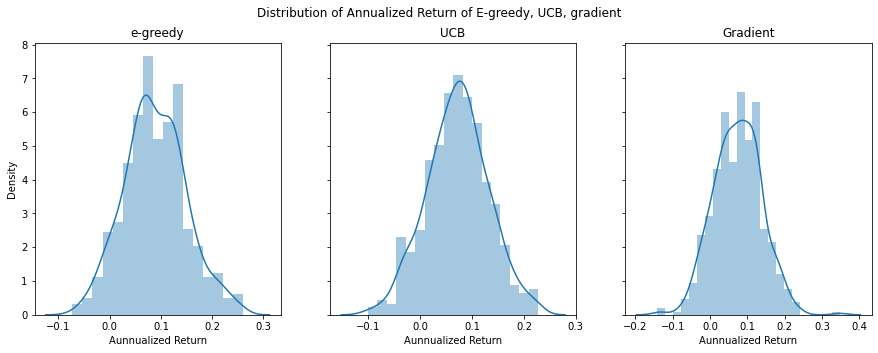
\includegraphics[width=.6\textwidth]{eu}
\end{center}
\caption{The distribution of returns on EU market}
\end{figure}

\section{Conclusion}
As the numerical result shows, these three MAB algorithms cannot outperform simple traditional trading strategies in both EU and US markets as we have expected. Hence we can conclude that the assumptions of the bandit problem violate the dynamic and rule of the stock market. Bandit takes less information from the market while normally we can know the stock return without investing in the stocks. There is no actual trade-off between exploration and exploitation in stock investing if we don’t consider slippage or any interaction with the market.
However, there might be other available methods to apply bandits algorithms on investing. For instance, we can regard different traditional strategies as different arms of a bandit. And the transaction cost is totally ignored on this project. We are willing to make improvements if we have further research opportunities.



\end{document} % inputs paper_content.tex


\printbibliography[title={References}]




\section{Acknowledgments}

This group assignment is completed by XU Guosong and CHEN Zuozhi with equal contribution. We had many times of video and face-to-face discussions about the whole idea. XU is responsible for collecting US market data, writing scripts for a part of MAB algorithms, and all the Momentum strategies. CHEN is responsible for collecting EU market data, modifying the rest of the MAB algorithms, and encapsulating them into a class. Then XU wrote the $\LaTeX$ code of this report while CHEN was running and checking the experiments parallelly.
Also, we would like to express our sincere appreciation to Professor Chak WONG and TAs because of their patient help.

\end{document}